\documentclass[10pt,landscape]{cheatsheet}

\usepackage{lipsum}
\usepackage{booktabs}
\usepackage[labelfont=bf,font=small]{caption}
\usepackage{fontspec}
\usepackage[pdfauthor={Luke Hsiao},
            pdftitle={Luke's Rubik's Cheatsheet},
            hidelinks]{hyperref}
\usepackage{datetime2}

\newcommand{\mitem}[2]{\textbf{#1} & \texttt{#2} \\}

\begin{document}
\footnotesize
\begin{multicols}{3}

\begin{center}
     \Large{\textbf{Rubik's Cheatsheet}}\\
     \scriptsize{Luke Hsiao, \today}
\end{center}

\section{Notation}
\begin{Figure}
    \centering
    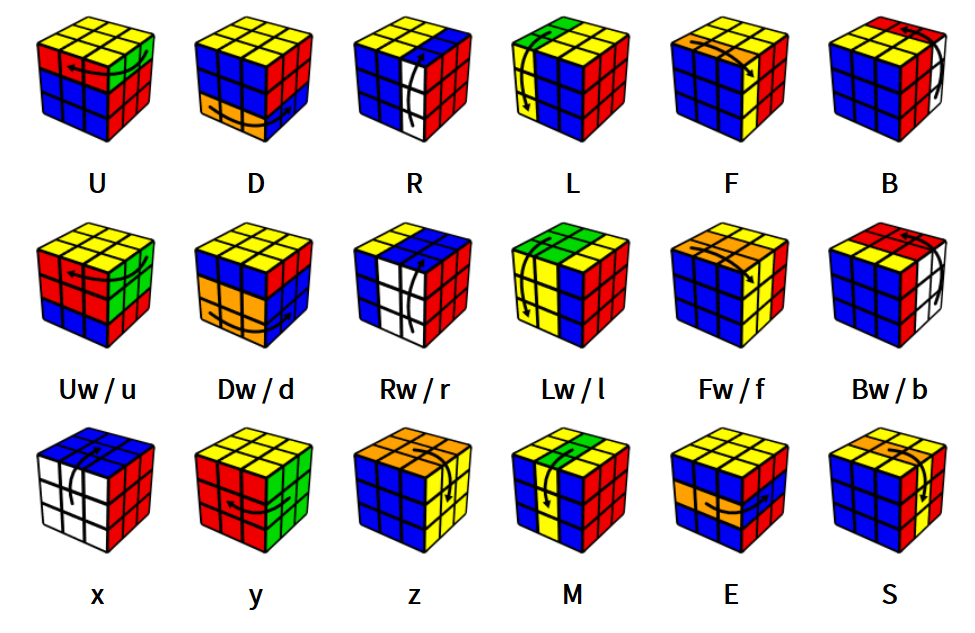
\includegraphics[width=\linewidth]{img/notation.png}
    \captionof{figure}{%
        Each notation corresponds to a clockwise turn if you were looking at the face.
        \texttt{M}, \texttt{E}, and \texttt{S} follow the face that they are closest alphabetically to.
    }\label{fig:notation}
\end{Figure}


\section{Beginner Method}

\begin{enumerate}
    \item Top cross
    \item Top corners
    \item 2nd row middles
    \item Bottom corners
    \item Bottom middles
\end{enumerate}

A good resource for scrambles and timing is \url{https://cstimer.net/}.

\subsection{Algorithms}

These algorithms are written with white side up (assuming you used white as your ``top'').
Also, these algorithm names are just arbitrarily chosen by me and are not standard.

\begin{tabular}{ll}
    \toprule
    \mitem{Right}{D' R' D R D F D' F'}
    \mitem{Left}{D L D' L' D' F' D F}
    \midrule
    \mitem{CornerRotate}{R' D' R D' R' D2 R D2}
    \mitem{CornerSwap}{R' D' R F D F' R' D R D2}
    \mitem{TwoTowers}{F L B' L' F' B D B D' B'}
    \mitem{CycleBreak}{M D' M' D2 M D' M'}
    \bottomrule
\end{tabular}

\vfill

\section{Roux Method}

One of the faster methods that is appealing due to it having a low average move count, being highly intuitive (thus requiring very few algorithms), and not needing reorientations.
Other popular methods are CFOP (most current world records are set using this) and ZZ.
Check \url{https://www.reddit.com/r/Cubers/wiki/best_methods} for a more detailed comparison.

\begin{enumerate}
    \item Left block of 6
    \item Right block of 6
    \item Top corners
    \item Top colors (arrow)
    \item Complete left and right faces
    \item Complete \texttt{M} slice
\end{enumerate}

\subsection{Algorithms}

These algorithms are written with yellow side up.
Yellow side up is often used for speed-cubing because you can more easily use your fingers to turn the cube quickly.

\begin{tabular}{ll}
    \toprule
    \mitem{Sune}{R U R' U R U2 R'}
    \mitem{J-Perm}{R U R' F' R U R' U' R' F R2 U' R'}
    \bottomrule
\end{tabular}

\end{multicols}
\end{document}
